\section{Durchführung}
\label{sec:Durchführung}

\begin{figure}
    \centering
    \begin{subfigure}{0.4\linewidth}
        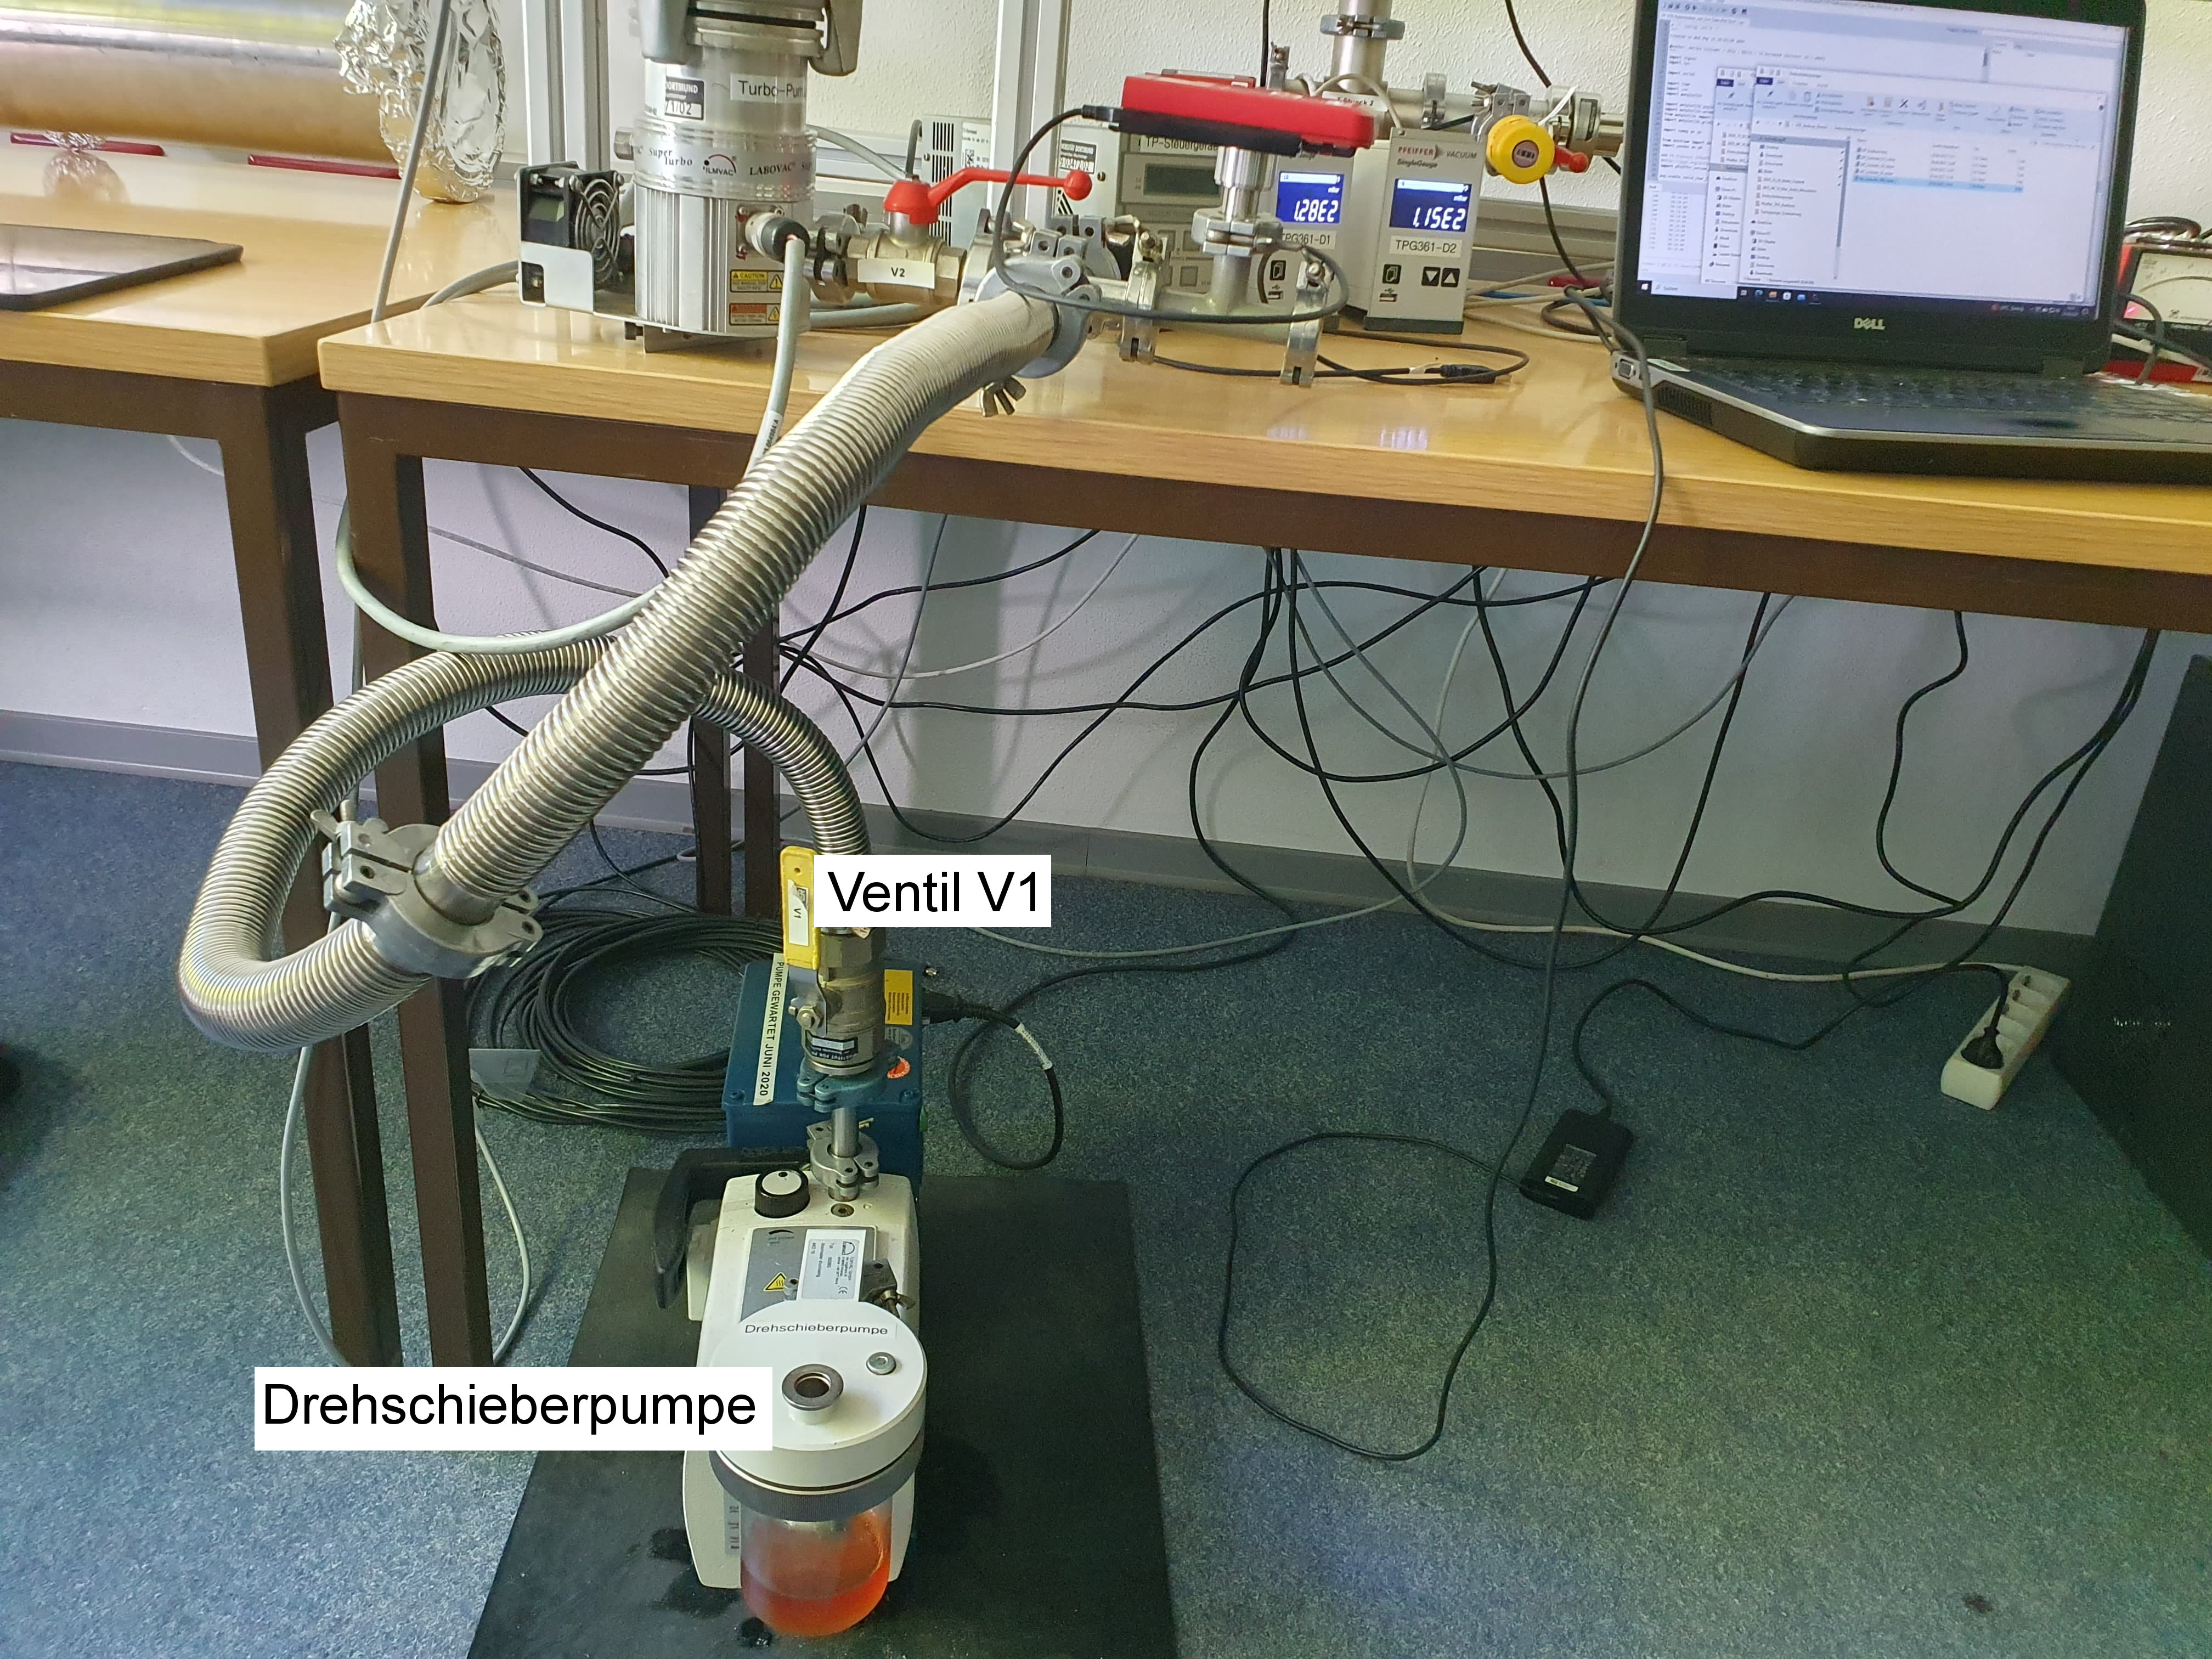
\includegraphics[width=\linewidth]{assets/V70_aufbau_2}
    \end{subfigure}
    \begin{subfigure}{0.4\linewidth}
        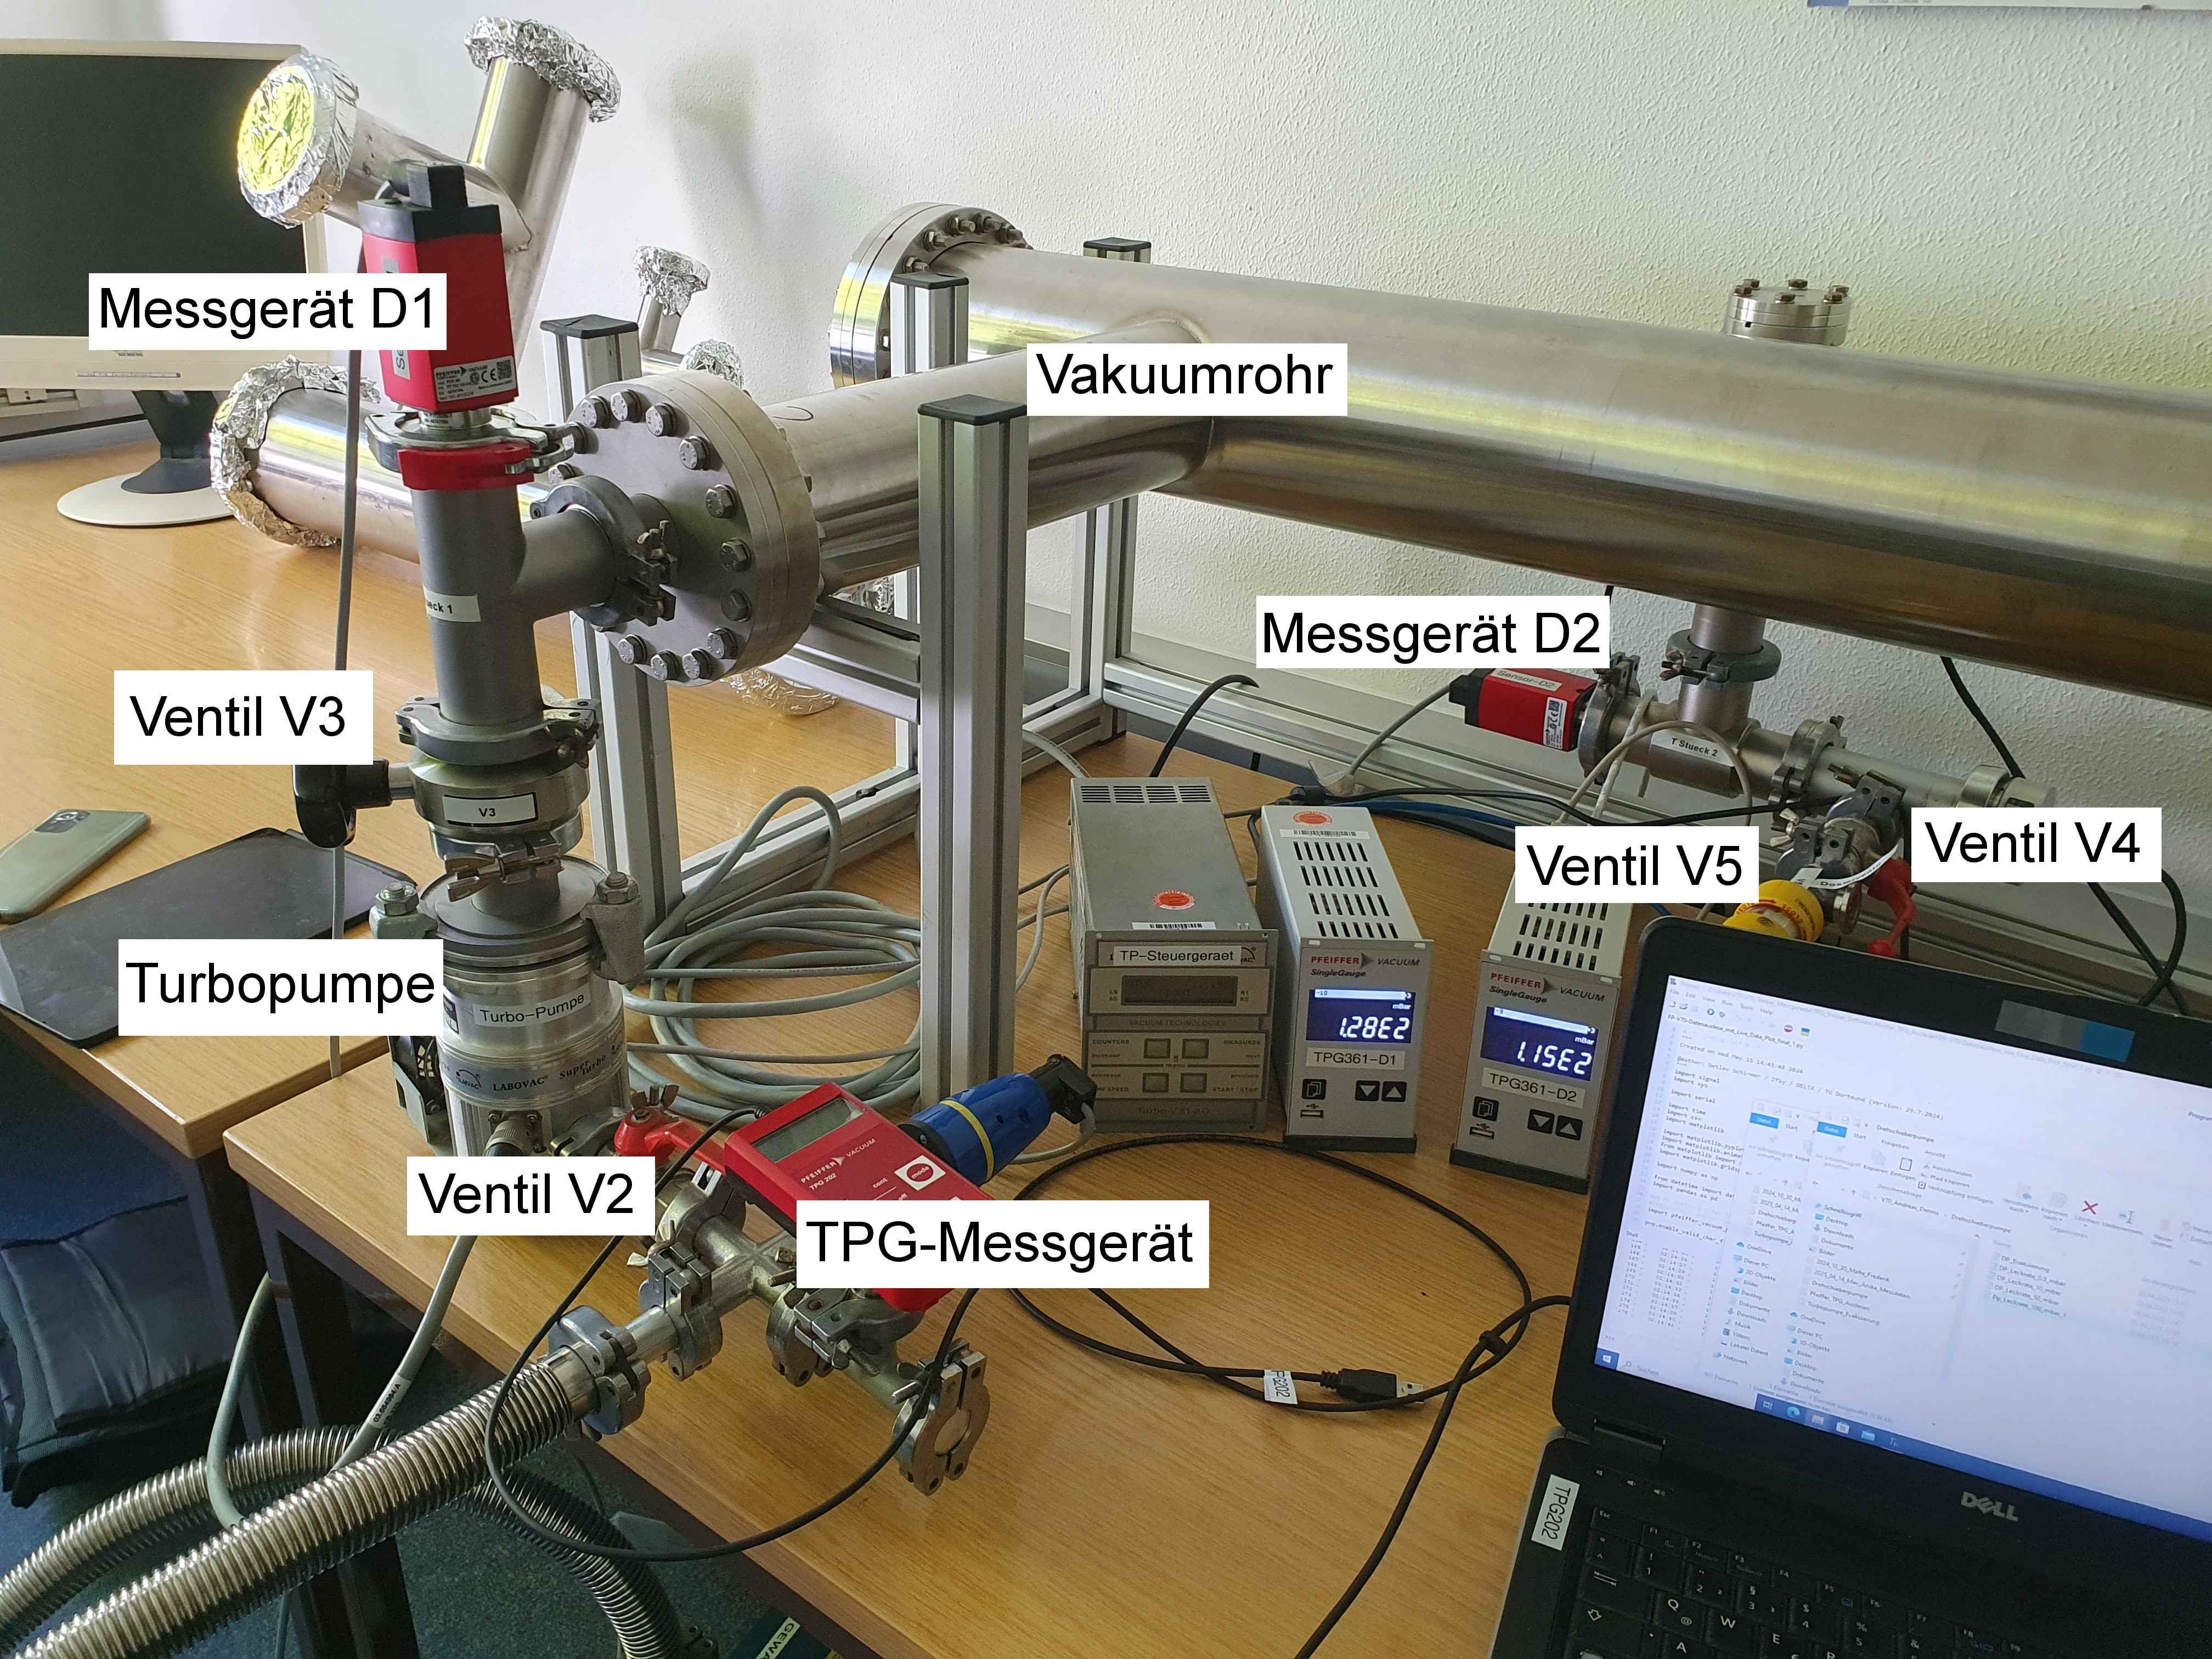
\includegraphics[width=\linewidth]{assets/V70_aufbau_1}
    \end{subfigure}
    \caption{Aufbau des Versuchs.}
    \label{fig:aufbau}
\end{figure}
Für den Versuch wird der in \autoref{fig:aufbau} dargestellte Versuchsaufbau genutzt.

\subsection{Evakierungskurve der Drehschieberpumpe}
In diesem Teil des Versuches wird nur die Drehschieberpumpe genutzt, die Turbopumpe bleibt vorerst ausgeschaltet.
Zunächst werden die Ventile V4 und V5 geöffnet, sodass der Rezipient vollständig gelüftet wird und sich bei laufender Drehschieberpumpe der Normaldruck von ca $\SI{1000}{mbar}$
in diesem einstellt.
Sobald dies geschehen ist wird das Skript zur Messung gestartet. Die beiden Ventile V4 und V5 werden möglichst zeitgleich geschlossen. Nun wird für eine Messzeit von etwa $\SI{600}{s}$
der Druck innerhalb des Rezipienten an dem TPG202-Messgerät ausgelesen. Nach Ablauf der Messzeit wird die Pumpe für weitere 5 Minuten laufen lassen und der sich eingestellte Enddruck
wird notiert. Diese Messung wird 1-mal durchgeführt.

\subsection{Leckratenmessung der Drehschieberpumpe}
Bei laufender Drehschieberpumpe und geöffneten Ventilen V1 und V4 wird das Dosierventil V5 teilweise geöffnet, so dass sich ein Gleichgewichtsdruck $p_{\mathit{g}}$ im Rezipienten einstellt.
Sobald der Gleichgewichtsdruck konstant bleibt wird das Skript zur Messung gestartet. Nun wird das Ventil V1 geschlossen, während die Ventile V4 und V5
geöffnet bleiben. Die Drucksteigerung wird über eine Messzeit von etwa $\SI{200}{s}$ am TPG202-Messgerät ausgelesen. Diese Messung wird für 4 verschiedene Gleichgewichtsdrücke
$p_{\mathit{g}} = 0.5; 10; 50; \SI{100}{mbar}$ durchgeführt. Die Messung für $p_{\mathit{g}} = \SI{100}{mbar}$ wird dabei 3-mal durchgeführt, die Messungen für die anderen Drücke jeweils 1-mal.

\subsection{Evakuierungskurve der Turbomolekularpumpe}
Nun wird zusätzlich zur Drehschieberpumpe auch die Turbomolekularpumpe eingeschaltet. Bei geöffnetem Ventil V4 wird über das Dosierventil V5 ein Vakuumdruck von $\SI{5e-3}{mbar}$ eingestellt.
Der Druck wird dabei am Messgerät D1 abgelesen.
Nun wird das Skript zur Aufnahme der Messdaten gestartet. Die Ventile V4 und V5 werden möglichst zeitgleich geschlosssen. Für eine Messzeit von etwa $\SI{120}{s}$ wird vom Messgerät
D1 der Druck innerhalb des Rezipienten ausgelesen. Die Turbopumpe wird für etwa 5 Minuten weiter laufen gelassen und der Enddruck wird aufgenommen.
Die Messung wird insgesamt 3-mal durchgeführt.

\subsection{Leckratenmessung der Turbomolekularpumpe}
Bei geöffnetem Ventil V4 und laufender Turbopumpe wird das Dosierventil V5 teilweise geöffnet, sodass sich ein konstanter Gleichgewichtsdruck innerhalb des Rezipienten einstellt.
Dann wird das Skript zur Messung gestartet und das Ventil V3 wird geschlossen. Der Druckanstieg wird über eine Messzeit von etwa $\SI{120}{s}$ am Messgerät D1 ausgelesen.
Die Messung wird für 4 verschiedene Gleichgewichtsdrücke $p_{\mathit{g}} = \num{5e-5}; \num{7e-5}; \num{1e-4}; \SI{2e-4}{mbar}$ jeweils 1-mal durchgeführt.

\subsection{Messung zum Leitwert}
Für diesen Teil des Versuches wird ein zusätzliches Testrohr mit kleinerem Querschnitt zwischen das Messgerät D1 und das große Vakuumrohr, wie in \autoref{fig:aufbau_leitwert}
dargestellt, eingebaut. Wie zuvor wird bei laufender Turbopumpe eine Leckratenmessung bei $p_{\mathit{g}} = \SI{1}{mbar}$ durchgeführt. Über eine Messzeit von etwa $\SI{120}{s}$
wird der Druck sowohl an D1 als auch bei D2 ausgelesen. Die Messung wird 1-mal durchgeführt.